% \appendix
\chapter{Appendix}
\section{Heuristic Rules from \cite{zhou-directive}}
\subsection{Not-null Heuristics}
\label{app:not-null}
\begin{table}[h]
	\centering
	\begin{tabular}{|c|c|}
		\hline
		\textbf{Rule} & \textbf{Nullness Not Allowed Heuristics (@exception or @throws)} \\ \hline
		1 & [something] be/equals null \\ \hline
		2 & [something] be equal/equivalent to null \\ \hline
		3 & [something1] or [something2] be/equals null \\ \hline
		4 & [something1] or [something2] be equal/equivalent to null \\ \hline
		5 & [something] parameter be null \\ \hline
		6 & The specified [something] be null \\ \hline
		7 & Any/none of [something] be null \\ \hline
		8 & Either/neither/any/all/both/none parameter(s) be/equals null \\ \hline
		9 & Either/neither/any/all/both/none parameter(s) be equal/equivalent null \\ \hline
		10 & Either/neither [something1] or/nor [something2] be/equals null \\ \hline
		11 & Both [something1] and [something2] be null \\ \hline
		12 & The [type] be null \\ \hline
		13 & [parameter phrase] be/equals null \\ \hline
		14 & [parameter phrase] be equal/equivalent null \\ \hline
		15 & [something]’s value be/equals null \\ \hline
		16 & [something]’s value be equal/equivalent null \\ \hline
		17 & Value of [something] be/equals null \\ \hline
		18 & Value of [something] be equal/equivalent null \\ \hline
	\end{tabular}
	\caption{Complete list of heuristic rules for exception nullness not allowed.}
	\label{tab:complete-not-null-heuristic-except}
\end{table}

\begin{table}[h]
	\centering
	\begin{tabular}{|c|c|}
		\hline
		\textbf{Rule} & \textbf{Nullness Not Allowed Heuristics (@param)} \\ \hline
		19 & [something] can not be null \\ \hline
		20 & Non-null [something] \\ \hline
	\end{tabular}
	\caption{Complete list of heuristic rules for parameter nullness not allowed.}
	\label{tab:complete-not-null-heuristic-param}
\end{table}

\subsection{Range Limitation Heuristics}
\label{app:range-limit}
\begin{table}[h]
	\centering
	\begin{tabular}{|c|l|}
		\hline
		\textbf{Rule} & \textbf{Range Limitation Heuristic (@exception or @throws)} \\ \hline
		1 & [something] >/</= [value] \\ \hline
		2 & [something] be \{not\} less/greater/larger/equal/equivalent than/to [value] \\ \hline
		3 & [something] equals [value] \\ \hline
		4 & \makecell{[something1] or/and [something2] be \{not\} \\ less/greater/larger/equal/equivalent than/to [value]} \\ \hline
		5 & \makecell{Computing [expression] be {not} \\ less/greater/larger/equal/equivalent than/to [value]} \\ \hline
		6 & \makecell{Computing either [expression1] or [expression2] be \\ \{not\} less/greater/larger/equal/equivalent than [value]} \\ \hline
		7 & \makecell{Product/sum of [something1] and [something2] be \\ {not} less/greater/larger/equal/equivalent than/to [value]} \\ \hline
		8 & [something] be {not} negative/positive/false/true \\ \hline
		9 & [something1] or/and [something2] be {not} negative/positive/false/true \\ \hline
		10 & [something1] and [something2] be {not} the same \\ \hline
		11 & [something1] equals [something2] \\ \hline
		12 & [something] be {not} in/out of/outside of range [range value] \\ \hline
		13 & [something] be {not} in/out of bounds \\ \hline
		14 & [something] be {not} [value] \\ \hline
		15 & [range expression] (only the expression,like ) \\ \hline
		16 & [something] be {not} between [value1] and [value2] \\ \hline
		17 & [something] be {not} [value set] \\ \hline
		18 & [something] be {not} one of [value set] \\ \hline
		19 & [something] be {not} one of following: [value set] \\ \hline
		20 & [something] be {not} one of supported data, which are [value set] \\ \hline
	\end{tabular}
	\caption{Complete list of heuristic rules for exception range limitations.}
	\label{tab:complete-heuristics-range-limit-except}
\end{table}

\begin{table}[h]
	\centering
	\begin{tabular}{|c|c|}
		\hline
		\textbf{Rule} & \textbf{Range Limitation Heuristic (@param)} \\ \hline
		21 & [something] can/must {not} be negative/positive/non-negative/non-positive \\ \hline
		22 & [something] must be greater/less/larger than [value] \\ \hline
		23 & [something] be greater/less/larger than [value] \\ \hline
	\end{tabular}
	\caption{Complete list of heuristic rules for parameter range limitations.}
	\label{tab:complete-heuristics-range-limit-param}
\end{table}

\section{Independent Study Contract}

\centering
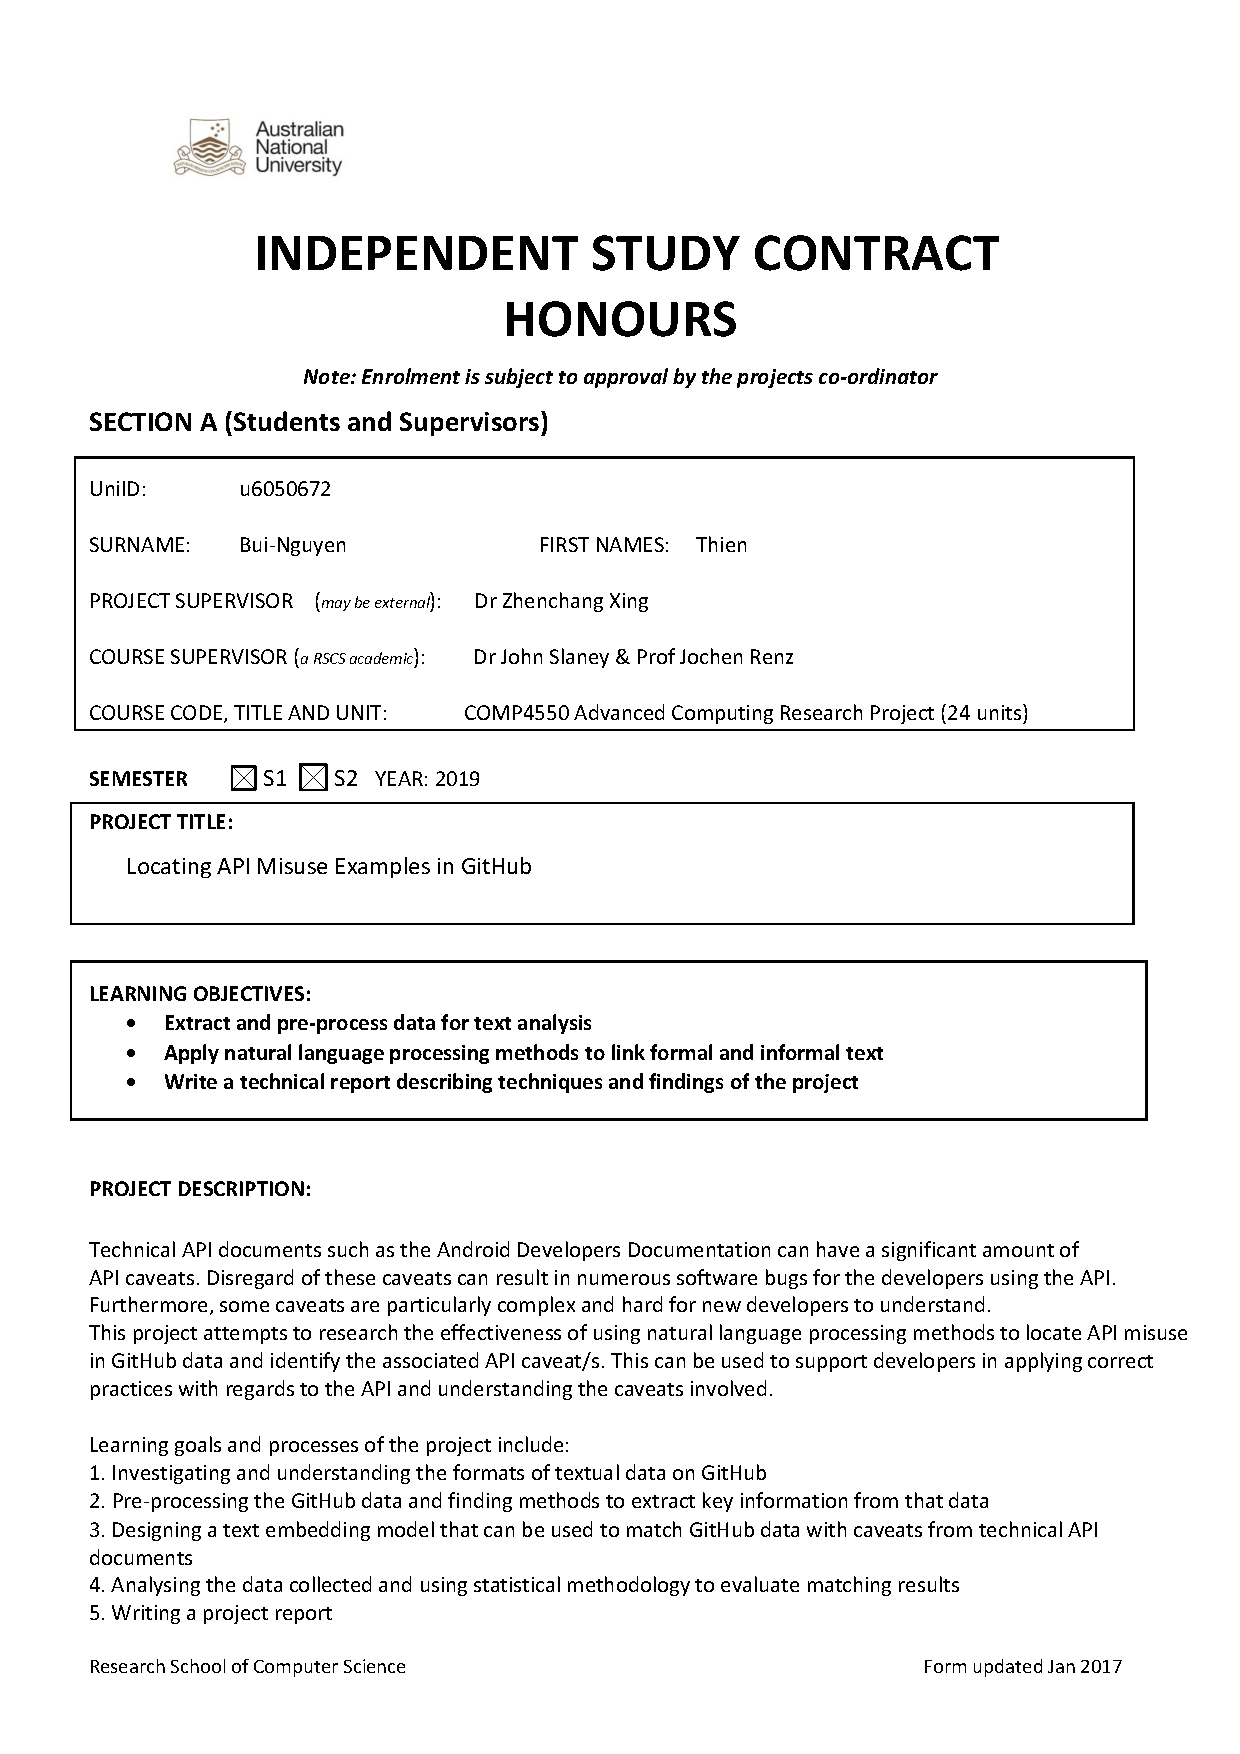
\includegraphics[page=1,width=0.8\textwidth]{figs/study-contract.pdf} \newpage
\includegraphics[page=2,width=0.8\textwidth]{figs/study-contract.pdf} \newpage

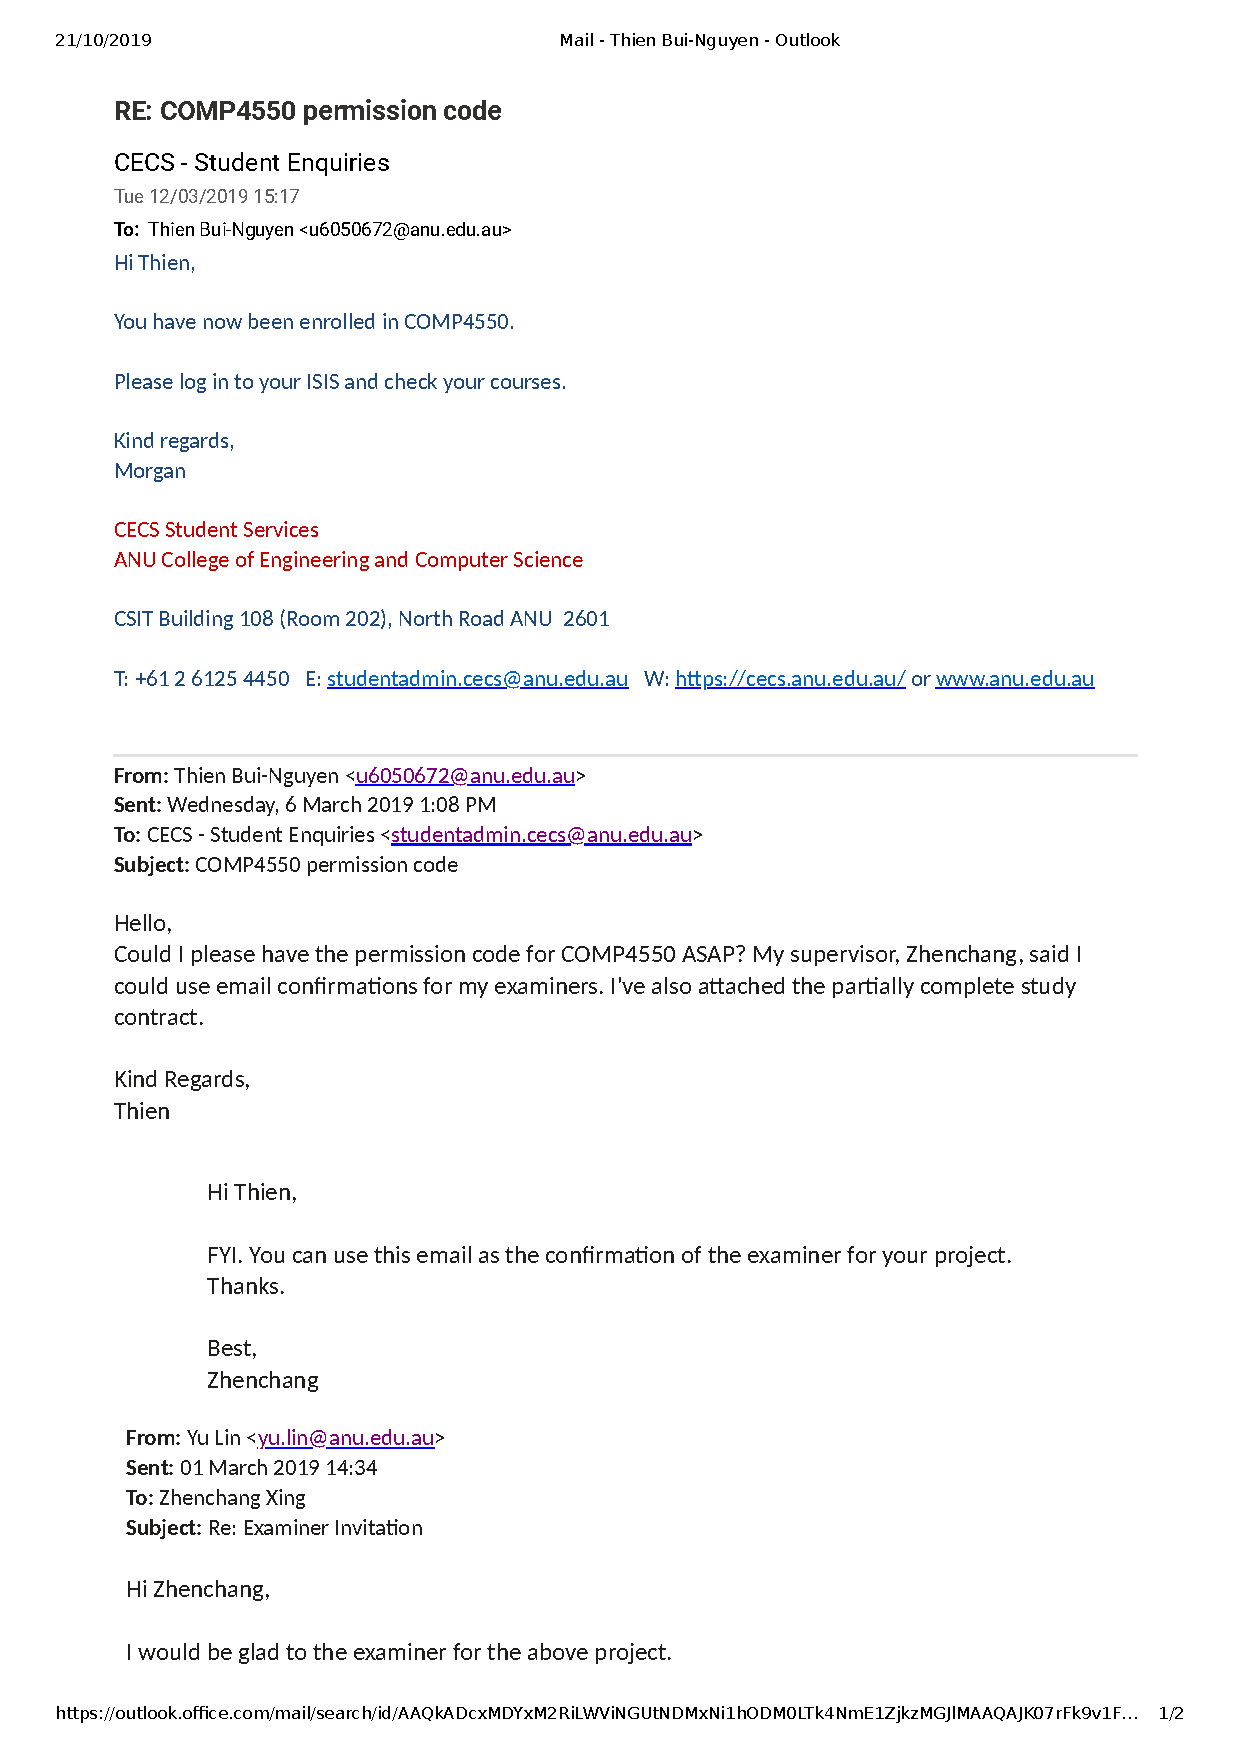
\includegraphics[page=1,width=0.8\textwidth]{figs/examiner.pdf} \newpage
\includegraphics[page=2,width=0.8\textwidth]{figs/examiner.pdf} \\
\flushleft